\subsubsection{Neural language models}
\label{sub:neural_language_models}

Neural networks avoid the curse of dimensionality problem (the number of possible sequences of words increases exponentially with the size of the vocabulary) that arises with language modeling by representing words in a distributed way, as a non-linear combination of weights.

One of the first solutions that comes to mind is the use of a \textbf{fixed window} neural language model. Similarly to an n-gram, the input of the neural network could be a context (window) around each word, but instead of counting n-gram frequencies the weights of the network are adjusted to optimize the output prediction in order to maximize the probability of the training corpus. This architecture foregoes the need of storing all possible n-grams. However, there are other problems that remain: Firstly, the fixed window will always be too small, there still is no way of processing inputs of arbitrary length. Secondly, there is no symmetry in the processing of outputs. This means that $ x^{(1)} $ and $ x^{(2)} $ are multiplied by completely different weights even though their output is most probably correlated. The idea of applying the same weight matrix repeatedly leads to a new architecture called \textbf{\gls{rnn}}.

\paragraph{Recurrent neural networks}
With their paper “Learning representations by back-propagating errors”~\footcite{10.5555/65669.104451} from 1986, David Rumelhart, Geoffrey Hinton and Ronald Williams laid the foundations for current \gls{rnn} architectures (figure~\ref{fig:recurrent_neural_network_architecture}. This work showed that these networks can learn an internal “hidden“ state - which is neither part of the input nor the output - that represents important features of the task domain. Unlike feedforward neural networks, RNNs can use their internal state (memory) to process \textit{variable length sequences of inputs}, which makes them so valuable for language modeling.

\begin{figure}[h]
  	\includegraphics[height=4cm]{img/rnn_structure}
  	\caption{Unrolled recurrent neural network}
	\label{fig:recurrent_neural_network_architecture}
\end{figure}

There are a few benefits that arise from the \gls{rnn} architecture. As the same weight matrix is used for every input, model size does not increase for longer input. Also, the model can process inputs of every length. And finally, this architecture allows for usage of information from the past and for symmetric input processing by using the same weight matrix. Because \gls{rnn}s synthesise and reconstitute the training data in a complex way they rarely generate the same thing twice. The predictions are “therefore much better at modelling real-valued or multivariate data than exact matches”~\footcite{DBLP:journals/corr/Graves13}.

[INPUT OF equations?? hidden states etc. stanford lecture 6 page 23]

The form of \gls{rnn} that has been described so far is known as the so called “vanilla RNN”. It is the most basic form of the \gls{rnn} class of artificial neural networks. Because of the heavy computations involved in adjusting the weight matrix vanilla \gls{rnn}s are susceptible to the problem of vanishing gradients. To tackle the shortcomings of vanilla \gls{rnn}s different \gls{rnn}-based architectures have been developed: LSTMs, GRUs and others.

It is worth inspecting the details of Long-Short Term Memory \gls{rnn}s, introduced in 1997 by Sepp Hochreiter and Jürgen Schmidhuber~\footcite{818041}, as their real-world usage has been crowned with success.

\bigskip

\paragraph{LSTMs}
In the last few years (2013-2016), big companies like Apple, Facebook, Google and IBM have been known to use \textbf{\gls{lstm}} based architectures in their products for translation and text generation with features like “smart reply” and “quicktype”~\footnote{\url{https://www.wired.com/2016/06/apple-bringing-ai-revolution-iphone/}, \url{https://ai.googleblog.com/2015/08/the-neural-networks-behind-google-voice.html}, \url{https://ai.googleblog.com/2015/09/google-voice-search-faster-and-more.html}, \url{https://ai.googleblog.com/2016/05/chat-smarter-with-allo.html}, \url{https://www.wired.com/2016/09/google-claims-ai-breakthrough-machine-translation/}, \url{https://www.zdnet.com/article/}, \url{ai-big-data-and-the-iphone-heres-how-apple-plans-to-protect-your-privacy/}, \url{https://www.allthingsdistributed.com/2016/11/amazon-ai-and-alexa-for-all-aws-apps.html}}. While \gls{rnn}s are theoretically able to learn long-term dependencies by choosing the parameters of the network in such a way that problems of this form can be solved, experience has shown that these networks ``expose a trade-off between efficient learning by gradient descent and latching on information for long periods''~\footcite{279181}. If we take a look at the task of predicting the next word given the following input
\begin{quote}
	When she tried to print her tickets, she found that the printer was out of toner. She went to the stationery store to buy more toner. It was very overpriced. After installing the toner into the printer, she finally printed her \_\_\_\_\_\_
\end{quote}
we see that the \gls{lm} needs to model the dependency between the word `tickets' on the $ 7^{th} $ step and the target word `tickets' at the end. In a \gls{rnn} the gradient (which can also be interpreted as the effect of the past on the future) would likely become so small over time that it would not be possible for the model to learn this dependency.

The underlying core concept of \gls{lstm}s is the introduction of the so called cell state in addition to the hidden state. This cell is used to store long-term information. The LSTM can hereby erase, write and read information from the cell. The selection of which information is erased, written or read is controlled by three corresponding gates called the forget, input and output gate. Before heading into the details, some basic terminology will be explained. On step $ t $, there is a hidden state $ h^{(t)} $ \textit{and} a cell state $ c^{(t)} $. Both are vectors of dimension $ n $. On each timestep, each element of the gates can be open (1), closed (0) or somewhere in-between - this value is dynamically computed based on the provided context. The calculation and meaning of the gates will be gone over on the basis of figure~\ref{fig:lstm_architecture}.
\begin{figure}
  	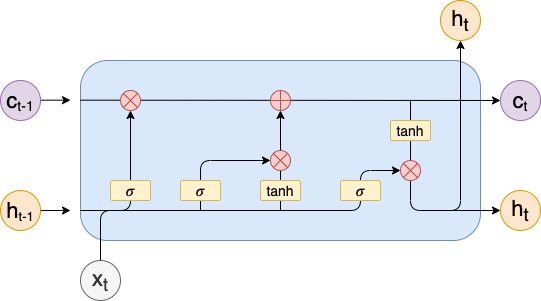
\includegraphics[height=6cm]{img/lstm}
  	\caption{Repeating module in an LSTM}
	\label{fig:lstm_architecture}
\end{figure}

In the first step, the \textbf{forget gate} (equation~\ref{eq:forget_gate}) determines what information is going to be disregarded for the calculation of the next output. In this case, the decision is made by a sigmoid layer ($ \sigma $). This layer looks at $ h_{t-1} $ amd $ x_t $, and outputs a number $ \in [0, 1] $ for each number in the cell state $ C_{t-1} $. If the gate is open (1), all the information from the hidden state should be kept.
\begin{equation}
	\label{eq:forget_gate}
	\pmb{f}^{(t)} = \sigma \left( \pmb{W}_f \pmb{h}^{(t-1)} + \pmb{U}_f \pmb{x}^{(t)} + \pmb{b}_f \right)
\end{equation}
The next step consists of two parts. First, the \textbf{input gate} (equation~\ref{eq:input_gate}) decides which values of the cell will be updated through the new cell content.
\begin{equation}
	\label{eq:input_gate}
	\pmb{i}^{(t)} = \sigma \left( \pmb{W}_i \pmb{h}^{(t-1)} + \pmb{U}_i \pmb{x}^{(t)} + \pmb{b}_i \right)
\end{equation}
Next, a tanh layer creates a vector of potential \textit{candidate values}, $ \widetilde{c}^{(t)} $, that could be added to the state (equation~\ref{eq:cell_candidates}).
\begin{equation}
	\label{eq:cell_candidates}
	\widetilde{\pmb{c}}^{(t)} = \text{tanh} \left( \pmb{W}_c \ \pmb{h}^{(t-1)} + \pmb{U}_c \ \pmb{x}^{(t)} + \pmb{b}_c \right)
\end{equation}
In order to now compute the updated cell state, equation~\ref{eq:new_cell_state} erases (``forgets'') some content from the last cell state, and writes (``inputs'') new cell content.
\begin{equation}
	\label{eq:new_cell_state}
	\pmb{c^{(t)}} = \pmb{f}^{(t)} \circ \pmb{c}^{(t-1)} + \pmb{i}^{(t)} \circ \widetilde{\pmb{c}}^{(t)}
\end{equation}
In the last step, the \textbf{output gate} controls what parts of the new cell content are written to the cell.
\begin{equation}
	\pmb{o}^{(t)} = \sigma \left( \pmb{W}_o \pmb{h}^{(t-1)} + \pmb{U}_o \pmb{x}^{(t)} + \pmb{b}_c \right)
\end{equation}
Based on that, the new hidden state is calculated.
\begin{equation}
	\pmb{h}^{(t)} = \pmb{o}^{(t)} \circ \text{tanh} \pmb{c}^{(t)}
\end{equation}
Besides \gls{lstm}s, researchers have proposed many gated \gls{rnn} variants. Another popular choice is the \textbf{\gls{gru}} architecture because it is quicker to compute and has fewer parameters than \gls{lstm}s. However, as there is no conclusive evidence that one consistently performs better than the other, \gls{lstm}s remain a popular default choice - especially when dealing with particularly long dependencies. For a few years, \gls{lstm}s where the dominant approach to building \gls{lm}s, but this approach has been replaced by a new architecture called `transformer' which will be presented in subsection~\ref{sub:attention_and_transformers}.

\bigskip

\paragraph{Convolutional neural networks}

CNNs are hierarchical networks in that convolution layers capture local contexts (Tang et al., 2018, p. 3). A parameterized multidimensional kernel is used to calculate a weighted average over a subset of input values. This is done by a stepwise shifting of a convolution matrix (filter kernel) over the input. The convolution operation for sequential data can be generalized by equation 3.6. The local context size depends on the size of the kernel and the number of layers. For a CNN with s layers and a kernel size k, the maximum context size (receiving field) is given by 𝑠(𝑘 - 1). For any two tokens in a local context with a distance of n the path length is equal to 𝑛/(𝑘 - 1). Since CCNs do not contain position information of the tokens, they are added encoded (𝑃𝐸𝑝𝑜𝑠,𝑖).
Bei CNNs wächst die Anzahl der Operationen, die erforderlich sind, um Signale von zwei beliebigen Ein- oder Ausgangspositionen zu beziehen (Tang et al., 2018, S. 3). Dieser Anstieg skaliert je nach Modell linear oder logarithmisch mit dem Abstand zwischen den Positionen (Vaswani et al., 2017, S. 1 f.). Dies erschwert das Erlernen von Abhängigkeiten zwischen entfernten Token und limitiert das Empfangsfeld (Dehghani et al., 2018, S. 1).